\section{Problemi durante lo sviluppo}

\subsection{Spring Boot}
I maggiori problemi che sono stati incontrati durante lo sviluppo di questa applicazione sono perlopiù relativi agli sforzi necessari per "immergerla" nel contesto di Spring Boot.\newline
Uno degli aspetti più critici è stata senza dubbio la configurazione della Web Security per l'applicazione, in parta dettata anche da una documentazione non sempre esaustive e/o aggiornata. Questo ha portato a diversi fallimenti nei test cases che sono stati man mano risolti con il procedere dell'applicazione e della conoscenza del framework stesso, un esempio ne è il seguente metodo:

\vspace{1cm}

\begin{minipage}{\linewidth}
	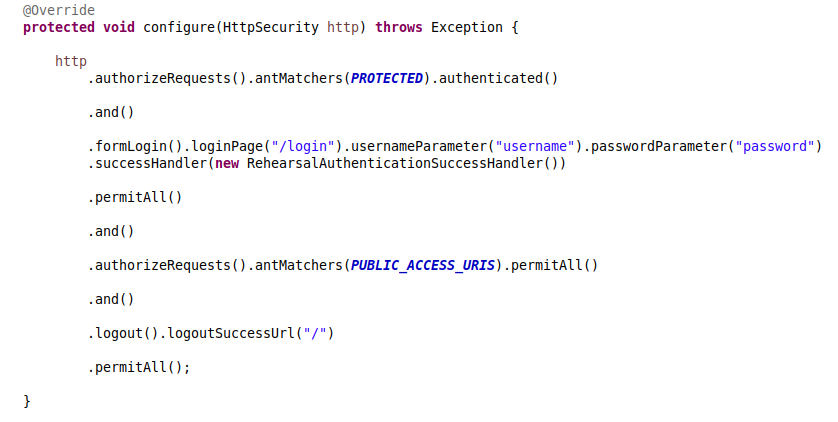
\includegraphics[width=\textwidth]{img/websecurity.png}
	\captionof{figure}{Metodi di configurazione per la web security. Configurarla in maniera appropriata richiede degli sforzi non indifferenti, sopratutto per capire quali sono gli strumenti a disposizione e come utilizzarli.\newline
	Gran parte del lavoro è svolta nel primo metodo, in cui vengono configurati le procedure di login, le richieste richiedenti autenticazione e quelle effettuabili in forma anonima.}
\end{minipage}

\vspace{1cm}

Un altro aspetto abbastanza problematico è stato l'utilizzo di un database per la gestione degli accessi degli utenti. È stato infatti necessario definire una classe che implementasse la classe Spring \textsl{UserDetailsService} per poter definire un \textsl{Bean} di tipo \textsl{DaoAuthenticationProvider} da utilizzare per l'autenticazione. Fortunatamente il problema è stato risolto abbastanza agilmente con il crescere della conoscenza del framework stesso.

\subsection{Gradle}

Passare dalla build-automation effettuata con Maven a quella di Gradle si è rivelato meno semplice del previsto, principalmente per l'enorme differenza con cui viene gestito il processo di build. Tuttavia, grazie a caratteristiche come un DSL per la specifica della build, Gradle si presenta piuttosto intuitivo in contrapposizione a Maven e l'xml.\newline
Uno degli aspetti più ostici è stato entrare nella mentalità di Gradle che impone una forte modularità nella definizione dei vari task personalizzati. È stato necessario studiare non solo in che modo i task vengono eseguiti ma anche come Gradle stesso gestisce le risorse (un esempio ne è la definizione delle classi e dei test case per i \textsl{SourceSets} presenti nei task \textbf{itest} e \textbf{e2eTest}).\newline\newline
Un altro aspetto che ha portato alcune problematiche nell'utilizzo di Gradle è stata indubbiamente la sua "novità" rispetto a Maven. Per quest'ultimo infatti sono presenti svariati tutorial e plugin ad-hoc per arricchire la build, per Gradle, essendo questo più giovane, risulta più difficile trovare materiale online.\newline
Un esempio calzante può essere la ricerca di un plugin per lanciare un immagine \textsl{Docker} (MongoDB) durante la build. La stragrande maggioranza dei plugin è progettata per \textbf{creare} un'immagine docker durante la build da caricare come docker image. È stato trovato un plugin che sembrava poter servire allo scopo prefissato ma, dal momento che utilizzava istruzioni di Gradle deprecate non è stato possibile usarlo, ragion per cui è stato scelto di utilizzare un plugin per avviare un server Mongo in-memory.